\chapter{Marco teórico}\label{ch:chapter_2}


\section{Código limpio}

\subsection*{Introducción histórica}
El concepto de Código Limpio ha sido fundamental en la programación de software desde los primeros días del desarrollo
de software, pero fue articulado y popularizado con gran efecto por Robert C. Martin en su libro~\cite{book_martin_2008}

Este libro se convirtió en una guía esencial para muchos desarrolladores al enfatizar la importancia de escribir código
que no solo funcione, sino que también sea fácil de entender, modificar y mantener.

\subsection*{Definición}
El código limpio es aquel que es fácil de entender y fácil de modificar y hace exactamente lo que se espera que haga.
Según Robert C. Martin, el código limpio puede ser leído y mejorado por un desarrollador que no sea su autor original
con un mínimo esfuerzo necesario.

Se caracteriza por su simplicidad, la ausencia de duplicación, la expresión clara de la intención del desarrollador y
la atención a los detalles en el nivel de código.


\section{Arquitectura limpia}

\subsection*{Introducción histórica}
En el ámbito del desarrollo de software, la arquitectura de un sistema es crucial para determinar su escalabilidad y
mantenibilidad a largo plazo.

Una de las metodologías que ha cobrado relevancia en este contexto son las ``arquitecturas limpias'', un enfoque para el
diseño de software promovido por Robert C. Martin en su libro Clean Architecture: A Craftsman`s Guide to Software
Structure and Design~\cite{book_martin_2017}

\subsection*{Definición}
La arquitectura limpia es un estilo de diseño que organiza el sistema de manera que sea independiente de los diferentes
elementos a los que considera detalles de implementación y que son intercambiables unos por otros:

\begin{itemize}
    \item frameworks
    \item interfaces
    \item bases de datos
    \item apis
\end{itemize}

La esencia de esta arquitectura radica en su diagrama de capas, donde cada capa tiene una responsabilidad claramente
definidas y depende solo de las capas más internas.
Esto se logra mediante el principio de inversión de dependencias, lo que significa que los detalles dependen de las
abstracciones y no al contrario.

Existen diferentes implementaciones de ``arquitectura limpia'', cada una con sus características intrínsecas, en este
proyecto hemos decidido implementar la versión en tres capas que aparece en la figura~\ref{fig:chapter_2.clean_architecture}.

\begin{figure}
    \begin{center}
        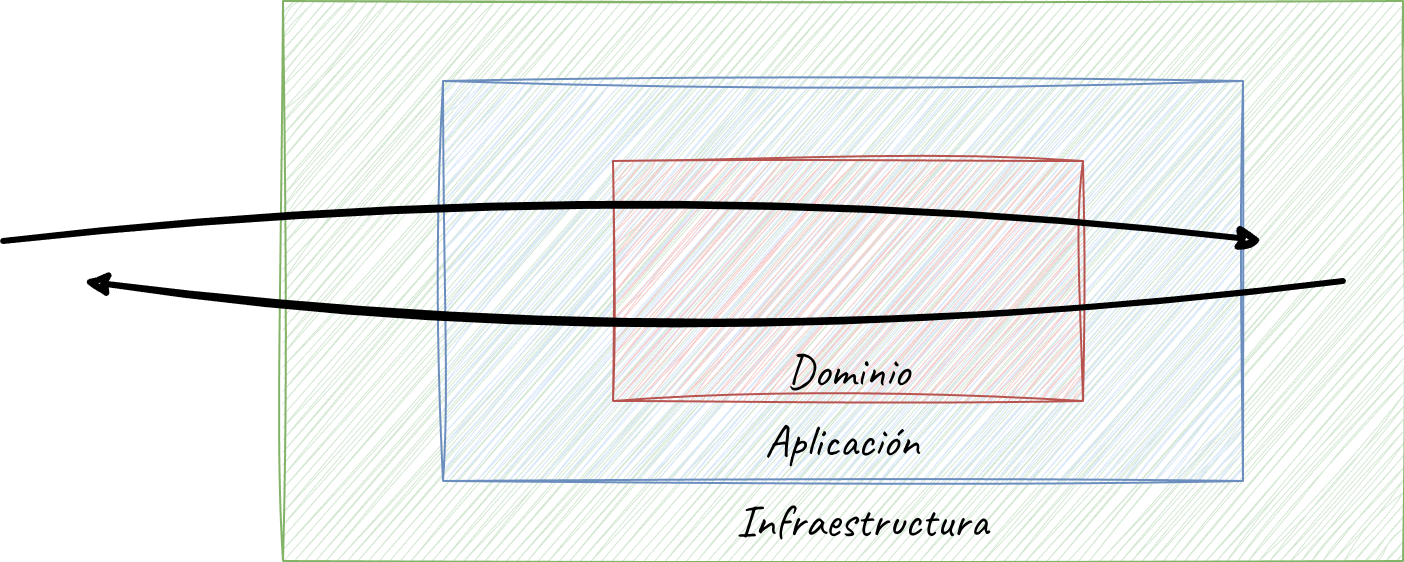
\includegraphics[width=0.5\textwidth]{chapter/2/images/chapter_2.clean_architecture}
        \caption{Esquema de una arquitectura limpia}
        \label{fig:chapter_2.clean_architecture}
    \end{center}
\end{figure}

La capa más interior se denomina \textbf{capa de dominio} y es el corazón del modelo de negocio de la aplicación y
encapsula la lógica y las reglas del negocio.
Esta capa es fundamentalmente agnóstica respecto a tecnologías externas y se centra exclusivamente en definir los
conceptos fundamentales del negocio.
Algunos de los elementos que puede contener son:
\begin{enumerate}
    \item entidades
    \item objetos de valor
    \item servicios de dominio
    \item abstracciones
\end{enumerate}

Esta capa debe ser autocontenida y fácilmente testable, aislada de tecnologías externas como bases de datos o
interfaces de usuario.

La capa que aparece a continuación es la \textbf{capa de aplicación}.
La capa de aplicación actúa como un mediador entre la capa exterior y la capa de dominio, coordinando las operaciones
de alto nivel que involucran múltiples aspectos del dominio.

La capa más exterior se denomina \textbf{capa de infraestructura}.
La capa de infraestructura proporciona las capacidades tecnológicas necesarias para que la capa de dominio puedan
realizar sus funciones sin tener que preocuparse por los detalles de implementación.
Toda la comunicación o interacción con elementos externos a la aplicación deben estar contenidos dentro de la capa de
infraestructura.


\section{Procesamiento de lenguaje natural}

\subsection*{Introducción histórica}
El Procesamiento de Lenguaje Natural o \textit{Natural Language Processing} (NLP) es un campo que se sitúa en la
intersección de la informática, la inteligencia artificial y la lingüística.

Se dedica al desarrollo de sistemas que permiten a las computadoras entender, interpretar y generar lenguaje humano de
una manera útil y significativa.
La historia del NLP comienza en la década de 1950, marcada por el trabajo pionero de Alan Turing y su famoso
test de Turing, que planteaba la cuestión de si una máquina puede emular el lenguaje humano de manera convincente
~\cite{article_touring_1950}.

En los años 60 y 70, el enfoque inicial estaba en la traducción automática, como los esfuerzos del proyecto
Georgetown~\cite{techreport_georgetown_1964}, mostró tanto promesas como limitaciones significativas, lo
que llevó a un reajuste en las expectativas~\cite{article_hutchins_2003}.

Con la introducción de la inteligencia artificial (IA) en la década de 1980, surgieron métodos basados primero en reglas
y luego en modelos estadísticos, culminando con el desarrollo de
modelos de aprendizaje automático~\cite{article_manning_1999} en la década de 1990.

El verdadero cambio paradigmático llegó con el advenimiento de las redes neuronales y el aprendizaje profundo en la
década de 2010.
Este período vio la creación de modelos de lenguaje avanzados~\cite{article_devlin_2019}, que han revolucionado la
capacidad de las máquinas para procesar el lenguaje con un grado de sutileza y profundidad sin precedentes.

\subsection*{Definición}

El NLP es un campo que combina técnicas de la informática, la inteligencia artificial y la lingüística computacional con
el objetivo de permitir que las máquinas entiendan, interpreten, manipulen y generen lenguaje humano de manera efectiva
y eficiente.

El NLP utiliza algoritmos y modelos matemáticos para abordar diversas tareas relacionadas con el lenguaje, tales como la
traducción automática entre idiomas, la generación de respuestas automáticas, la extracción de información relevante de
textos, el análisis de sentimientos, el reconocimiento de voz, y la síntesis de habla, entre otros.


\section{Modelos de lenguaje de gran escala}

\subsection*{Introducción histórica}
La historia de los Modelos de lenguaje de gran escala o \textit{Large Language Models} (LLMs) comienza con los
primeros modelos estadísticos de lenguaje en la década de 1980, que utilizaban métodos simples como los modelos de
Markov y n-gramas para predecir la probabilidad de secuencias de palabras~\cite{article_jelinek_1997}.

Estos métodos, aunque efectivos para algunas tareas básicas, estaban limitados por su incapacidad para capturar
contextos más largos y por su dependencia de grandes corpus de texto para entrenamiento.

En la década de 2000, con el advenimiento de modelos más sofisticados como los modelos ocultos de Markov y especialmente
las redes neuronales, comenzó a vislumbrarse el potencial de los modelos de lenguaje más complejos.

Sin embargo, no fue hasta la introducción de las redes neuronales recurrentes o \textit{recurrent neural networks} (RNN)
y, más tarde, las redes neuronales de memoria a largo plazo o \textit{long-term memory neural networks} (LSTM) que
los investigadores pudieron abordar el problema del ``desvanecimiento del gradiente'' y mejorar significativamente la
capacidad de los modelos para aprender dependencias a largo plazo en el texto~\cite{article_hochreiter_1997}.

El verdadero cambio paradigmático llegó en 2017 con el desarrollo de la arquitectura \textit{Transformer}
~\cite{article_vaswani_2017}.
Esta arquitectura introdujo el mecanismo de atención, que permite a los modelos ponderar diferentes partes de la entrada
de texto de manera dinámica, mejorando la capacidad de los modelos para manejar secuencias de texto largas y complejas.

\subsection*{Principales modelos}

\subsubsection*{GPT}
GPT o \textit{Generative Pre-trained Transformer} es un avanzado modelo de lenguaje desarrollado por OpenAI
~\cite{article_brown_2020}.
Es uno de los modelos más reconocidos en la actualidad.
Aunque es un modelo privado, OpenAI ofrece acceso a través de una API de pago que incluye una capa gratuita limitada.
GPT ofrece varios modelos, cada uno con un esquema de precios que varía según su complejidad.
Una de las principales ventajas de este servicio es que proporciona una solución integral \textit{plug-and-play}, es
decir, no requiere instalación ni configuración adicional por parte del usuario.

\subsubsection*{BERT}
BERT, desarrollado por Google~\cite{article_devlin_2019}, es un modelo de lenguaje basado en la arquitectura
\textit{Transformer} que se entrenó utilizando un gran corpus de texto en una manera bidireccional, lo que le permite
entender el contexto de una palabra basada en todas sus apariciones en un texto.

\subsubsection*{Hugging Face's Transformers}

\textit{Hugging Face's Transformers} es una biblioteca de NLP~\cite{article_wolf_2020} que simplifica el uso de modelos
de aprendizaje profundo basados en la arquitectura \textit{Transformer}.

Esta biblioteca ofrece una amplia variedad de modelos preentrenados y libres desarrollados por la comunidad para fines
específicos, además de la posibilidad de entrenar modelos personalizados.

En contraposición, los modelos disponibles en Hugging Face suelen ser menos potentes que los modelos más disponibles a
través de plataformas como GPT de Open AI~\cite{url_chat_gtp_vs_hugging_face_2024}.

\subsubsection*{Otros}

Además de los descritos existen muchas otras plataformas que ofrecen modelos LLM para desarrolladores interesados en
incorporar capacidades avanzadas de procesamiento de lenguaje natural en sus aplicaciones.
